\subsubsection{Timeouts with {\tt tile\_pos} and {\tt median}}
\label{sec:histograms}
Here we report the histograms of timeouts for the {\tt tile\_pos} and {\tt median} reference functions.
%
Please refer to Figures~\ref{fig:clamp_hist},~\ref{fig:tilepos_hist} and~\ref{fig:median_hist}.
%
\begin{figure}[ht]
    \centering
    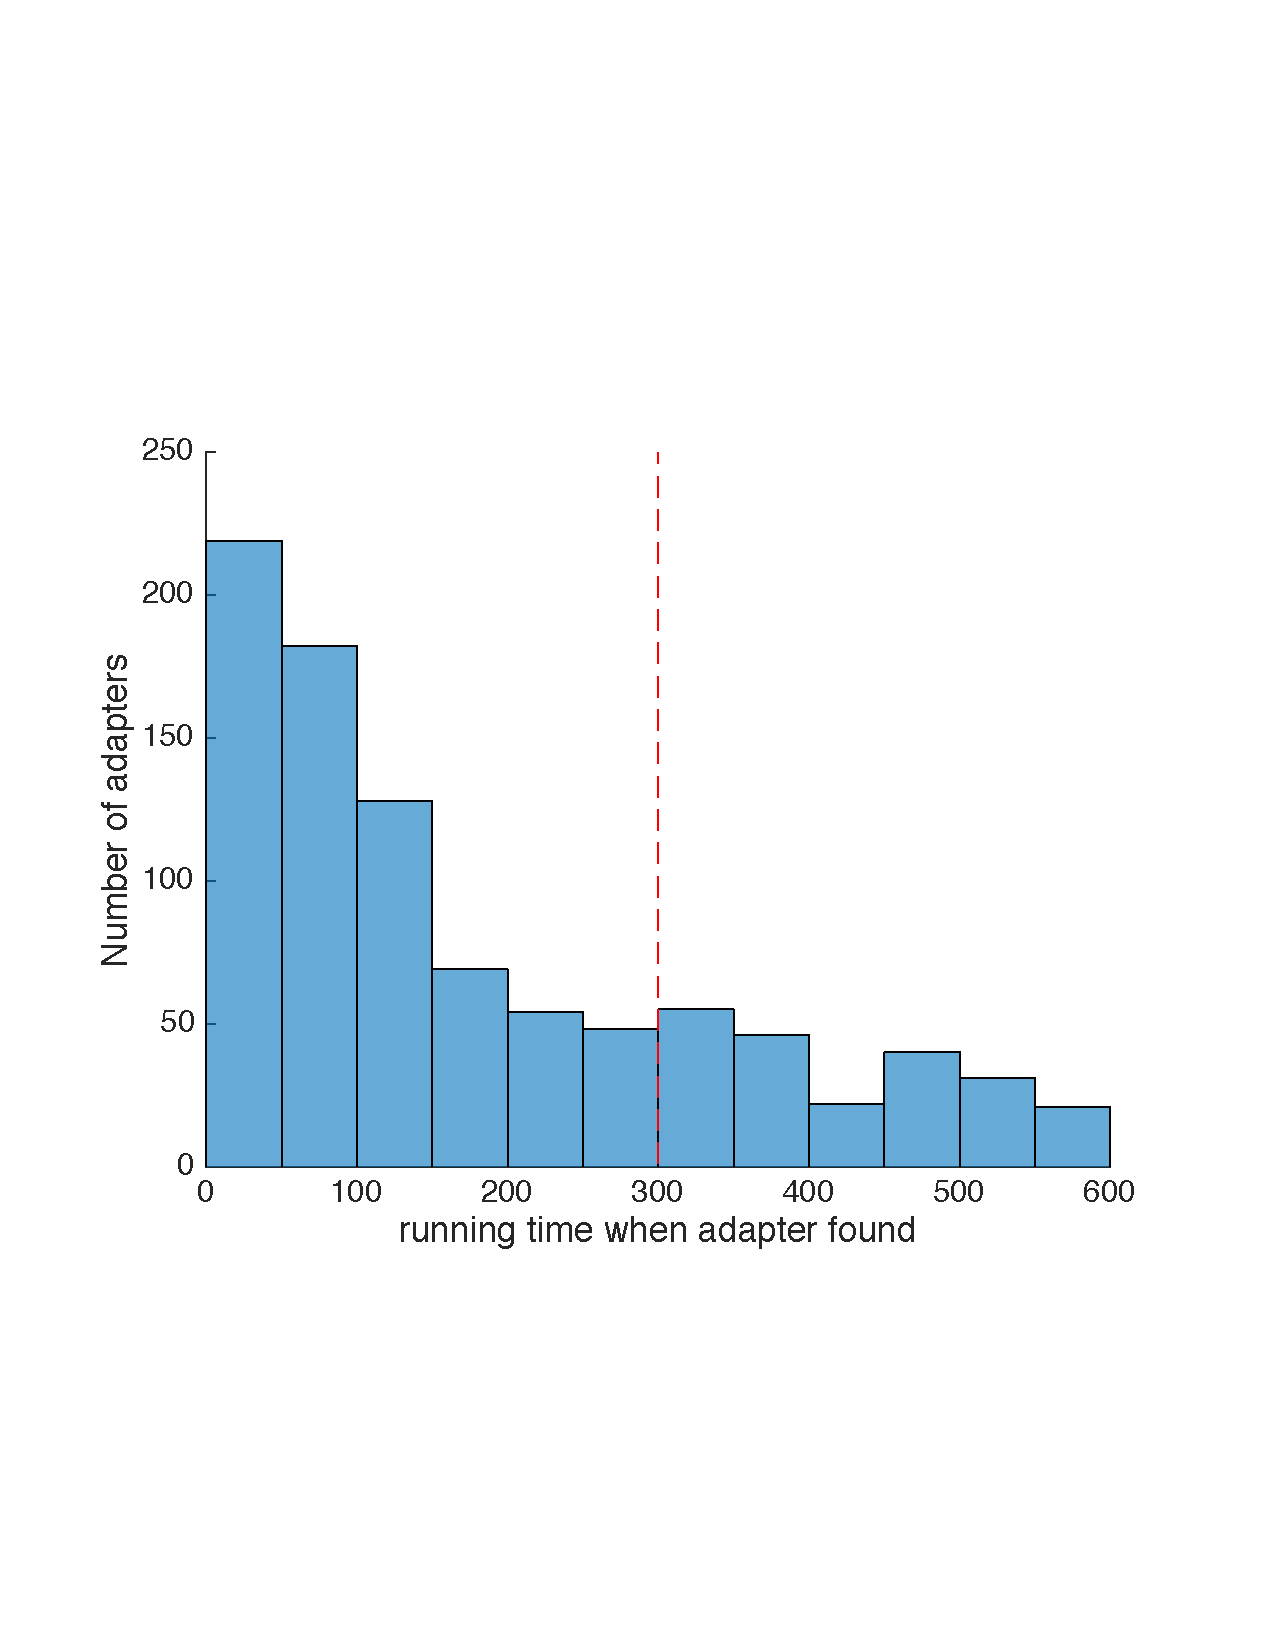
\includegraphics[width=\widthfactor\textwidth]{chapters/adapter_synthesis/figures/clamp_hist}
    \caption{Running times for synthesized adapters using {\tt clamp} reference function}
    \label{fig:clamp_hist}
\end{figure}
\begin{figure}
    \centering
    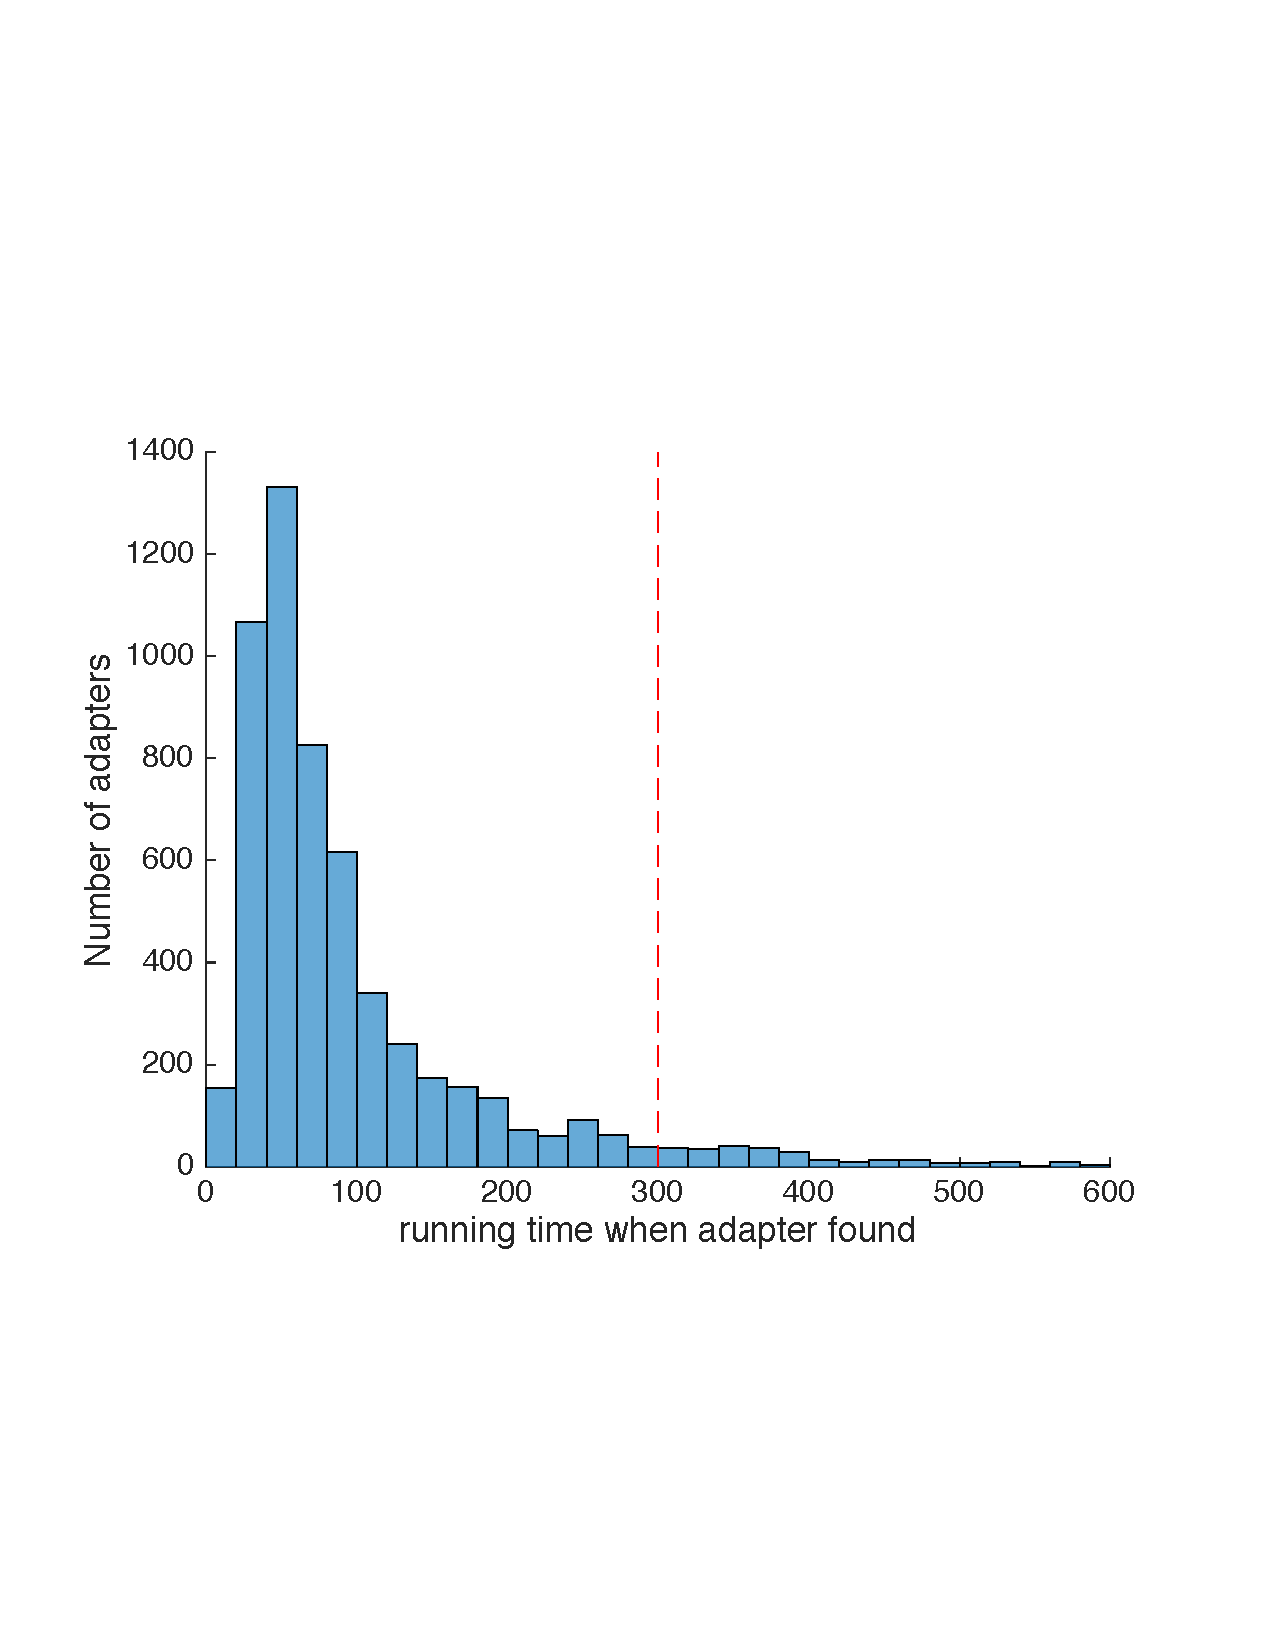
\includegraphics[width=\widthfactor\textwidth]{chapters/adapter_synthesis/figures/tilepos_hist}
    \caption{Running times for synthesized adapters using {\tt tile\_pos} reference function}
    \label{fig:tilepos_hist}
\end{figure}
%
\begin{figure}[ht]
    \centering
    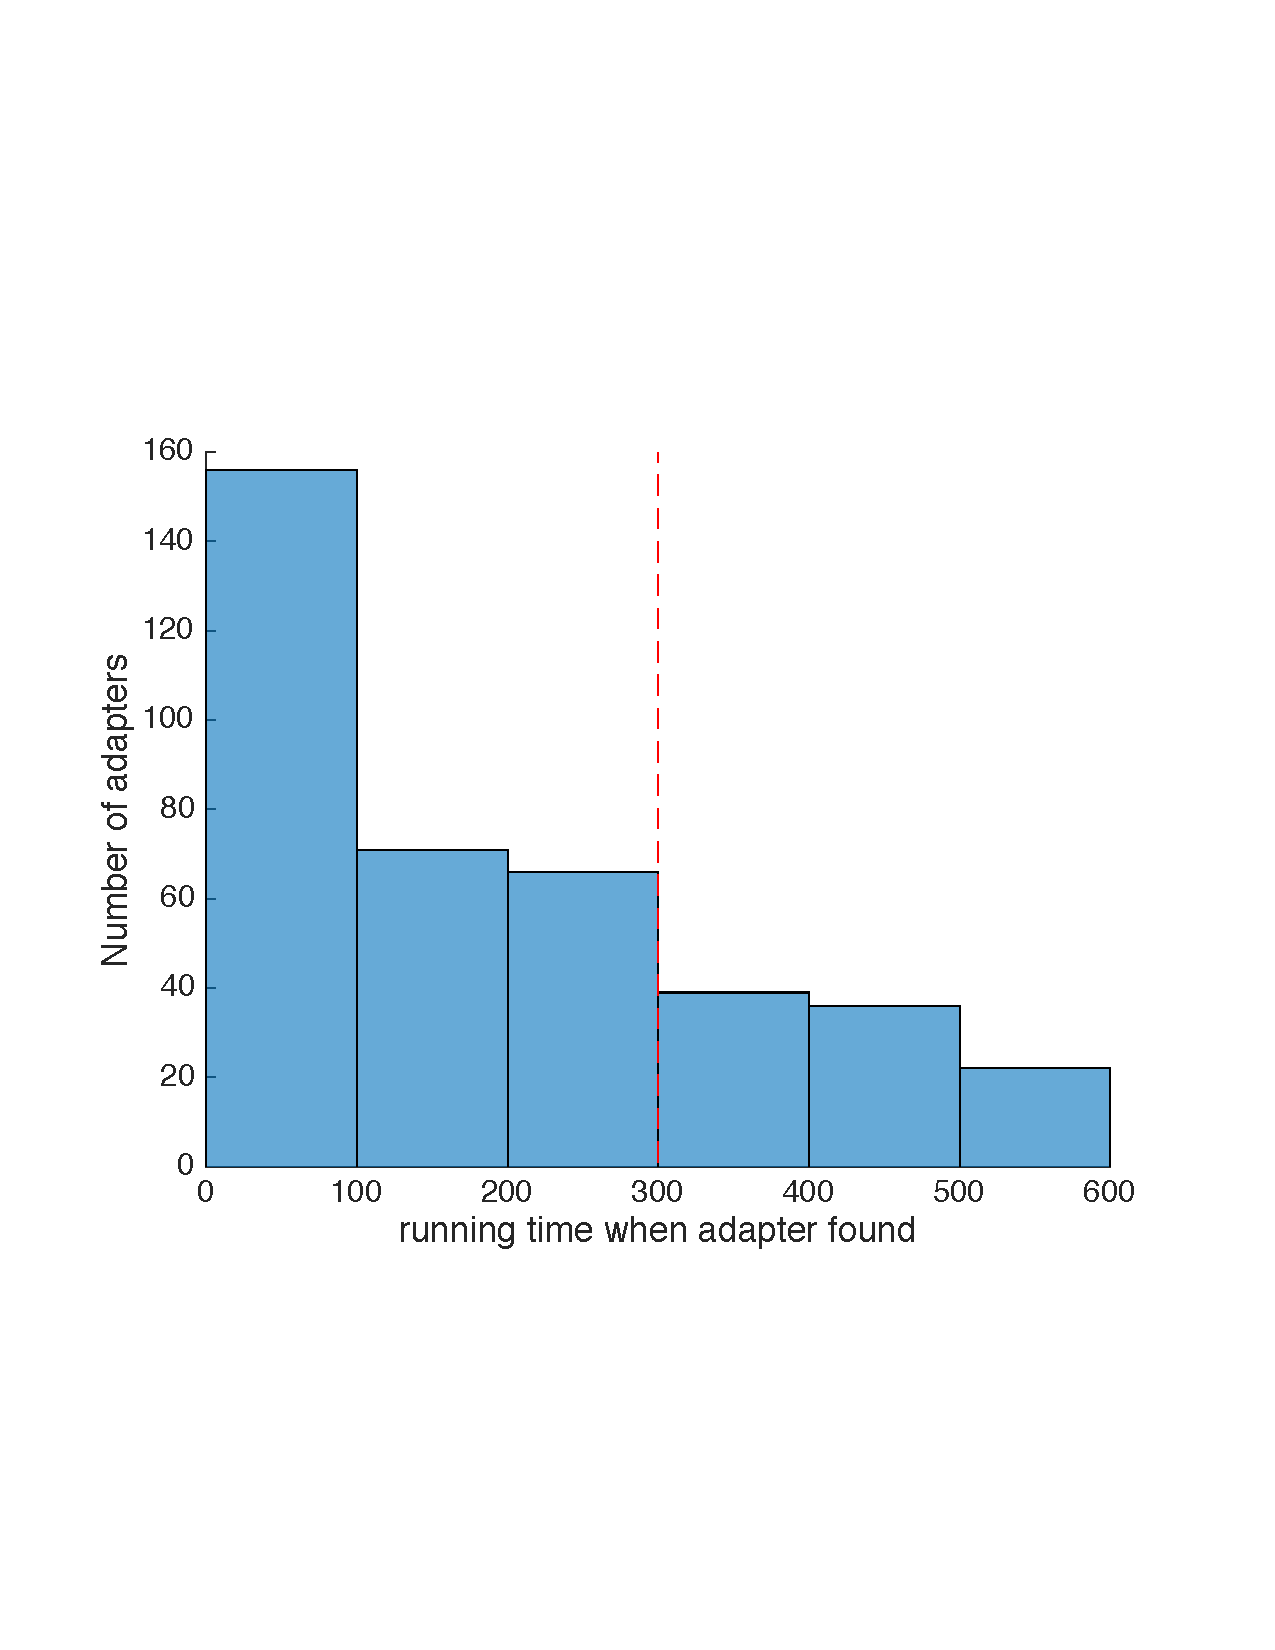
\includegraphics[width=\widthfactor\textwidth]{chapters/adapter_synthesis/figures/median_hist}
    \caption{Running times for synthesized adapters using {\tt median} reference function}
    \label{fig:median_hist}
\end{figure}
%
The number of adapters found after 300 seconds decreases rapidly, consistent with the mean total running time~(subcolumn \textit{total time} under column \textit{adapter} in Table~\ref{table:general}) of 99.3 seconds for the {\tt clamp} reference function.
%
Table~\ref{table:general} also shows that the total running time, when our tool concludes with finding an adapter, is significantly less than 300 seconds for all reference functions that reported adapters.
%
Though setting any finite timeout can cause some instances to be lost,
these results suggest that a 300-second timeout was appropriate for
this experiment, and that most timeouts would not have led to adapters.